\documentclass[a4paper,10pt]{article}

\usepackage[english]{babel}
\usepackage[utf8]{inputenc}
\usepackage{graphicx}
\usepackage{amsmath,amssymb}
\usepackage{hyperref, url}
\usepackage{tikz}
\usepackage{caption}
\usepackage{subcaption}


\parindent 0mm
\parskip 3mm

% add your name and student number in parenthesis
\title{T-61.5020 Statistical Natural Language Processing  \\ Topic and Sentiment analysis}

\author{Sergio Isidoro (410111)\\
	   \textit{Aalto School of Science} \\ \textit{Department of Information and Computer Science}\\ 	   
       {\tt sergio.isidoro@aalto.fi}}

\begin{document}

\maketitle

\section{Introduction}



\section{Task 1}

The data was mostly pre-processed in python, with resource to nltk.\

The first step was to read the file, and count the occurrence of each stem in the document, using the The Lancaster Stemming Algorithm of the nltk package. At the same time a counter of the global occurrence of the stems globally was kept.

At the same time, all english stop words were removed 

The vectors with the absolute count of stems in each document was the exported to matlab, and a matrix with the absolute count of stems was used to create a relative frequency of the stems ($OccorenceInDocument/GlobalOccurence$), as an intermediate step to further analysis. There was no normalization of the words not found in a document, meaning that the relative frequency of the words that don't appear in a document is zero. There was significant amount of cleaning to be done, since in the stems there were words such as "157224223x". To solve this problem, all columns that had one occurrence of a relative frequency bigger than 0.50 (50\% of some word appeared in one document alone), the feature (in this case, word), was removed. This resulting in cutting down by half the dimension of the vectors by removing the very unusual words that appeared just a few times on the data set.

Normalization in terms of the length of the document might not be suitable to the requested task. Since the task is topic analysis, the topic related words might be likely to appear just once or twice in the text, unlike stop-words and general verbs that will most likely by influenced by the length of document due to repetition. A certain word might appear in document A of length x and in the document B of length 2x - Both words may have equal impact on the topic. However, by not doing this, the document length will most likely appear as the first principal component, as the size of articles will introduce a lot of variance to the data. A choice was made to check two different approaches: First, use the relative frequency of the words in the document, followed by Principal Component analysis and K-means with euclidean distance, and the other, using binary vectors (word present /not present) and k-means using the hamming distance for comparing documents.

\section{Frequentist Approach}
For the frequentist approach, the word matrix is composed of the probabilities of, by randomly choosing a word from the article, to be a certain word, with zero in case of a word not being in the text. The most common verbs and subjects (such as I and you) will probably have low variance, and by computing the Principal Component Analysis, that aims to select the dimensions that explain the most variance, will have low impact on the clustering algorithm. 

After applying Principal Components, the projection of the articles onto the first 2 and 3 principal components are show in figure \ref{fig:pca}


\begin{figure}[h!]
        \centering
        \begin{subfigure}[b]{0.5\textwidth}
                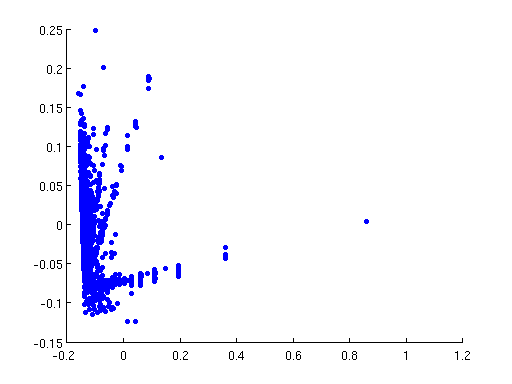
\includegraphics[width=\textwidth]{Images/processed.png}
                \caption{2 first principal components}
    			\label{fig:pca2}
        \end{subfigure}%
        ~ %add desired spacing between images, e. g. ~, \quad, \qquad etc.
          %(or a blank line to force the subfigure onto a new line)
        \begin{subfigure}[b]{0.5\textwidth}
                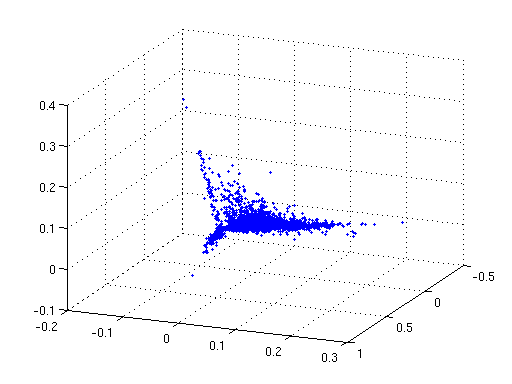
\includegraphics[width=\textwidth]{Images/pca3d.png}
                \caption{3 first principal components}
                \label{fig:pca3}
        \end{subfigure}
        \caption{Projection onto the the first principal components after pre processing}
        \label{fig:pca}
\end{figure}

There are some distinct branches coming out of the main cloud of articles. Those might be the topic clusters we are looking for. 

The results of the k-means clustering are shown in figure \ref{fig:cluster}

\begin{figure}[h!]
        \centering
        \begin{subfigure}[b]{0.4\textwidth}
                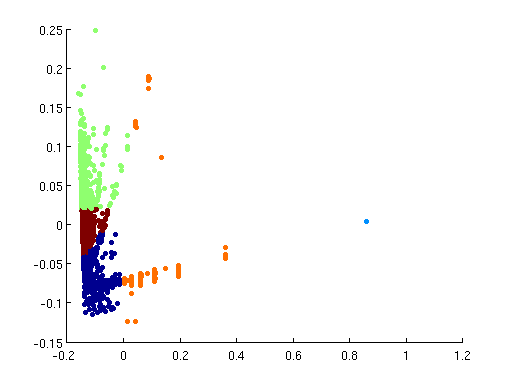
\includegraphics[width=\textwidth]{Images/classified1.png}
                \caption{Euclidean}
    			\label{fig:euclidean}
        \end{subfigure}
        ~
		\begin{subfigure}[b]{0.4\textwidth}
                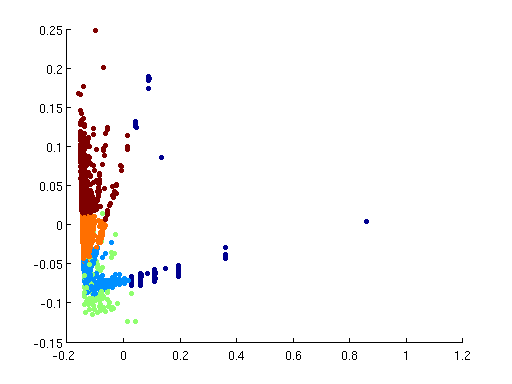
\includegraphics[width=\textwidth]{Images/cosine.png}
                \caption{Cosine Distance}
    			\label{fig:cosine}
        \end{subfigure}     
                                    
        \begin{subfigure}[b]{0.4\textwidth}
                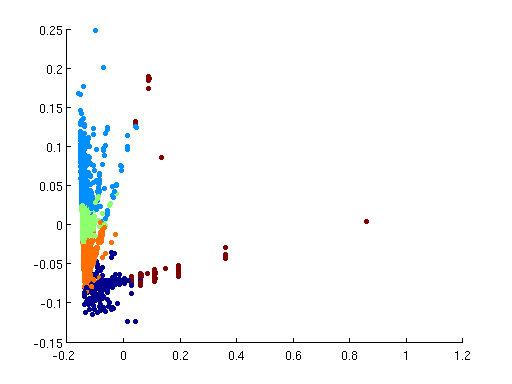
\includegraphics[width=\textwidth]{Images/correlation.png}
                \caption{Correlation}
    			\label{fig:correlation}
        \end{subfigure}
		~        
        \begin{subfigure}[b]{0.4\textwidth}
                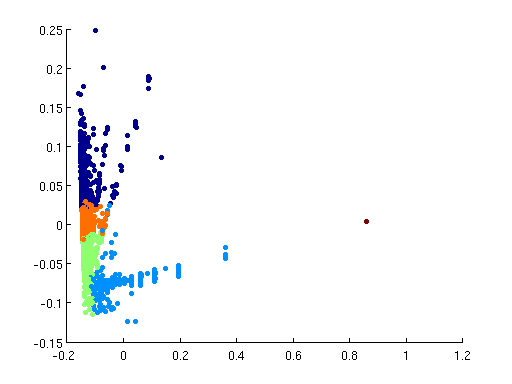
\includegraphics[width=\textwidth]{Images/cityBlock.png}
                \caption{City Block}
    			\label{fig:cityBlock}
        \end{subfigure}%  
        \caption{Culstering results}  
        \label{fig:cluster}
\end{figure}

The k-means algorithm does not seem to perform particularly well in the above setup, specially because there seems to be some sort of segmentation of the space in diagonal lines of the space, while k-means will search for spherical or square segmentation of the space (depending on the distance function). Yet, it seems by exploration of the plots of the principal components that the cosine distance gives out relatively better results than other distance measures.



\section{Binary Approach}
The binary approach consists of having only a word as "present" or "not present" and using the hamming distance for the clustering of the data. After the clustering, the classification was both projected onto the PCA of all the data (no pre-processing or normalization) and the PCA of the data after the cleaning mentioned in the previous section.

The results are shown in the figure \ref{fig:binary}
\begin{figure}[h!]
        \centering
        \begin{subfigure}[b]{0.4\textwidth}
                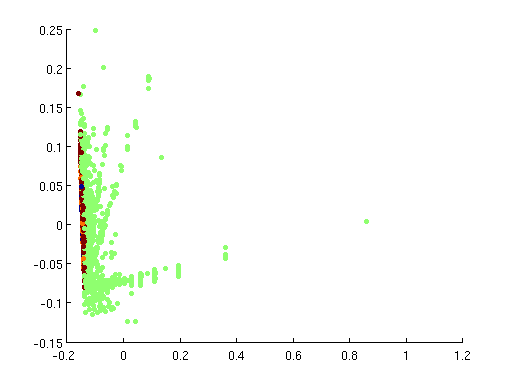
\includegraphics[width=\textwidth]{Images/hamming.png}
                \caption{Hamming distance of cleaned data onto PCA of cleaned data}
    			\label{fig:binary1}
        \end{subfigure}
        ~
		\begin{subfigure}[b]{0.4\textwidth}
                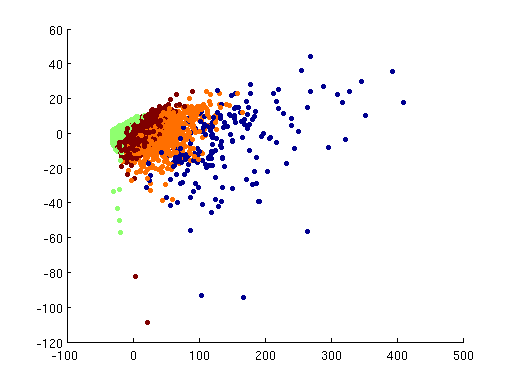
\includegraphics[width=\textwidth]{Images/HammingDistanceOriginal.png}
                \caption{Hamming distance of cleaned data onto PCA of all data}
    			\label{fig:binary2}
        \end{subfigure}     
        \caption{Binary data culstering}  
        \label{fig:binary}
\end{figure}

It seems that the hamming distance might be too sensitive to the document length, as a document that is longer, tends to have different new words, this increasing the distance between the documents. 

The PCA of all data, without any processing will probably tend to select as it's first principal components the underlying size of the document. It is seen on figure \ref{fig:binary2} that the hamming distance clustering is consistent with space defined by those same principal components (probably size of the sample), giving strength to those assumptions.

This approach doesn't seem appropriate to the task at hand.

\end{document}